\section{Summary}

The work within previous chapters have demonstrated the power of lens modeling as a tool for uncovering the mysteries of the high redshift universe. The Frontier Fields lens models have provided the community with easily-accessible lensing information of all the clusters for a variety of researchers regardless of their own expertise in lensing. Many of the papers in the literature, including that of the work in Chapter~\ref{chap:hff_clusters}, have been cited over 100 times since the models were released in 2014 \citep{Johnson:2014tg,Richard:2014gf}. This work includes greatly improving constraints on the faint end of luminosity functions at $z\sim6$ \citep {Bouwens:2017df} as the luminosity function up to $z\sim10$ \cite{Ishigaki:2017le,Ishigaki:2015cs,McLeod:2016xw}. Additional studies include characterizing the size distribution of these high redshift galaxies \citep{Kawamata:2017bc, Bouwens:2017to,Kawamata:2015ax}, as well as work on the clusters themselves, including intracluster light \citep{Montes:2018hs,Montes:2014jx,Morishita:2017zf} and dark matter substructure \citep{Natarajan:2017qp,Jauzac:2016dn,Mohammed:2016bk,Grillo:2016jk}. Another exciting discovery has been Supernova Refsdal, which was multiply-imaged into an Einstein cross in a galaxy at $z\sim1.5$ by both the cluster \MACSeleven\ and one of its galaxies \citep{Kelly:2016az,Rodney:2016sf,Kelly:2015pj}. With the lens models, astronomers were able to accurately predict a supernova \citep{Treu:2016lr,Jauzac:2016ux,Sharon:2015xe,Oguri:2015hb} -- Refsdal reappeared in another image of the galaxy roughly a year later \citep{Kelly:2016hw}.

We have seen, in Chapter~\ref{chap:ares_systematics} that due to the wealth of constraints and spectroscopic information, the Frontier Fields lens models are less vulnerable to systematic errors in derived magnifications \citep{Johnson:2016rt}. When marginalizing over the results produced by different modeling techniques, scientists can account for the systematic errors in the modeling methods themselves \citep{Meneghetti:2016xe}. \citet{Acebron:2017wl} also find that cosmological parameters can be retrieved from lens models of clusters similar to the Frontier Fields.

We have also seen how lensing clusters can magnify background galaxies to allow for unique, high resolution studies of galaxies at $1<z<3$. We saw in the modeling of \cluster\ that it is possible to break the kiloparsec, even the centaparsec resolution barrier in a galaxy at $z\sim2.5$. This result has major implications for understanding the morphologies of galaxies at cosmic noon. \citet{Rigby:2017qy} show that if \giantarc\ had been observed with \hst\ in a survey such as CANDELS or even in the HUDF, it would not be classified as a ``clumpy" galaxy as we see it lensed. We see with lensing that roughly a quarter of the star formation in \giantarc\ occurs in what we classify as clumps, where as in the hypothetical case this galaxy were observed in a deep field, we would see all the star formation occurring in an exponential disk (see Figure~\ref{chap6:fig:candelized}).

\begin{figure}
\centering
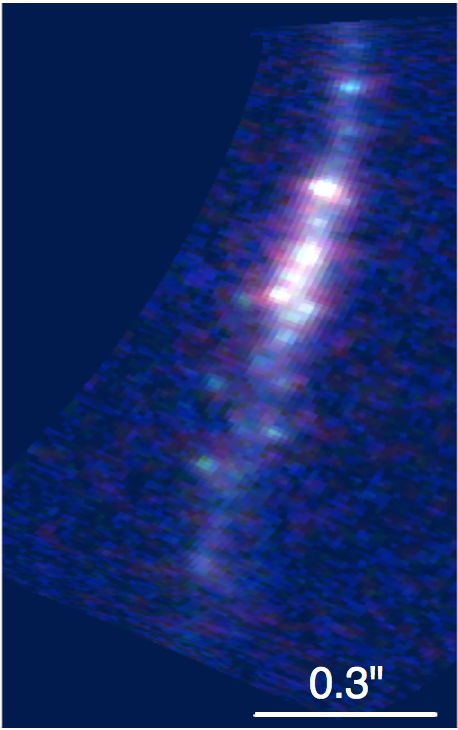
\includegraphics[height=0.4\textheight]{Chap6/candelized_highres.png}
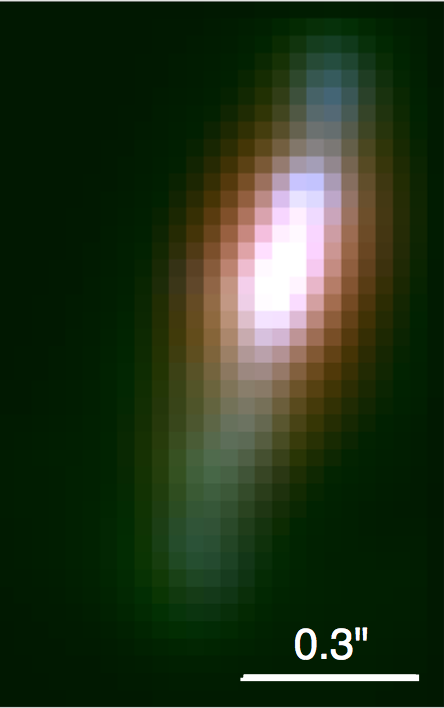
\includegraphics[height=0.4\textheight]{Chap6/candelized_lowres.png}
\caption[Comparison of lensed \giantarc\ source reconstruction to its unlensed deep field realization]{From \citet{Rigby:2017qy}: (left) The source plane reconstruction of \giantarc, pixel scale of 3 mas. Roughly 24\% of the star formation of this galaxy is in clumps. (right) \giantarc\ source reconstruction convolved with the \hst\ PSF and rebinned to a pixel scale of 30 mas. This is what this galaxy would look like had it been detected in a deep field. All the star formation would be observed to occur in an exponential disk, with no evidence of clump morphology.}
\label{chap6:fig:candelized}
\end{figure}

\section{Future of cluster lensing}

The Frontier Fields are only six unique sight lines to some of the best lensing clusters in the sky with full wavelength coverage in imaging and spectra. Despite their usefulness in characterizing the formation of galaxies into the era of cosmic re-ionization and understanding systematics of lens modeling techniques, the future of lensing will not depend on a handful clusters, but rather thousands.

\subsection{Clusters in future surveys}

As mentioned before, several hundreds of strong lensing clusters have already been discovered in ground-based optical surveys like SDSS and DES as well as in optical follow-up by surveys such as ROSAT, Planck, ACT, and SPT. The vast majority of these clusters have been discovered based on their high magnifications of background objects into discernible giant arcs. As on-going studies of these lensing systems are taking place, the astronomical community is greatly anticipating the first light from several new ground- and space-based optical observatories. The Large Synoptic Survey Telescope \citep[LSST; ][]{IVezic:2008tv} is expected to have first light in 2020 and will likely find hundreds of strong lensing clusters as it images entire southern sky every few nights. The National Aeronautics and Space Administration (NASA) plans to launch the Wide Field Infrared Survey Telescope \citep[WFIRST; ][]{Spergel:2013zk}, a 2.4-m infrared space telescope that will survey much of the sky and plans to find $>$40,000 galaxy clusters, but with roughly the same resolution as \hst. WFIRST is currently on-track to be launched in the 2020s. A complementary mission to WFIRST in the optical will be the European Space Agency's (ESA) {\it Euclid} telescope \citep{Laureijs:2011qt}, a 1.2-m telescope with a launch date planned for 2021. {\it Euclid} plans to identify $\sim10^5$ strong lensing systems.

\subsection{Modeling the lenses found in surveys}

\section{Systematic errors for clusters with few constraints}


